% Chapter Template
\chapter{4 Tensor Decomposition} % Main chapter title
\label{Chapter4}
\def \path	{Figures/C4}

In this chapter the main mathematical tools for the manipulation of tensors are introduced. 
Following, we will see how to apply these operators to decompose a convolutional layer through two different techniques, effectively exploring the state-of-the-art methods of low-rank approximation presented in the previous chapter.  

%--------------------------------------------------------------------
%	SECTION 1
%--------------------------------------------------------------------
\section{Background}}
%% intro 

%% SVD Applied on Fully Connected layer 

$$ (U_{n \times t}\Sigma_{t \times t}V^T_{m \times t})x + b $$ = $$ U_{n \times t} ( \Sigma_{t \times t}V^T_{m \times t} x ) + b $$


%--------------------------------------------------------------------
%	SECTION 2
%--------------------------------------------------------------------
\section{Tensor mathematical tools}

\subsection{Basic operations}
Before diving into tensor decomposition algorithms, let's define some fundamental tensor operations: 

\begin{itemize}
    \item  \textbf{Tensor times matrix: \textit{k}-mode product:} 
            The $k$-mode product of a tensor X $\in \mathbb{R}^{I_{1} \times I_{2} \times \ldots \times I_{N}}$ with a matrix $M \in \mathbb{R}^{J \times I_{k}}$ is written as: 
           \begin{equation}
                \textbf{Y} = \textbf{X} \times_{k} M
           \end{equation}
            The resulting tensor $Y$ is of size $I_{1} \times \ldots \times I_{k-1} \times J \times I_{k+1} \times \ldots \times I_{N}$, and contains the elements:

            $$ 
             y_{i_{1}  \cdots  i_{k-1}  j  i_{k+1}  \cdots  i_{N}} =   \sum_{i_{k} = 1}^{I_{k}} x_{i_{1}  i_{2}  \cdots  i_{N}} a_{ji_{k}}.
            $$
             
             It can be hard to visualize this operation at first, but effectively it boils down to 
             multiply each mode-\textit{k} fiber of X by the matrix M. Looking at \ref{fig:unfolding}, we can also represent the same operation with 
             $ \textbf{Y}_{(i)} = \textbf{X}_{(i)} \cdot M$, being $X_{(i)}$ the mode-i unfolding of the tensor X. \newline
             
             To simplify things, let \textbf{X} be a 3-mode tensor $\in F^{I \times J \times K}$ and $M$ a matrix $\in F^{N \times J}$, the k-mode product on axis 1 of X and M is:
            
            \begin{equation}
                        \textbf{Y} = \textbf{X} \times_{1} M, Y \in F^{I \times J \times K} 
            \end{equation}
            So each element (\textit{n, j, k}) of Y is obtained by: 
            \begin{equation}
                y_{n,j,k} = \sum_{i} x_{i,j,k}  \cdot  b_{n,j}  
            \end{equation}
            
            A visual example is depicted in \ref{k-mode}.

    
    \item \textbf{Tensor times vector}: 
       Given the same matrix X, the tensor-vector multiplication on the \textit{i}-axis is defined as:
       \begin{equation}
           \textbf{Y} = \textbf{X} \times_1 v, \textbf{Y} \in \mathbb{}
       \end{equation}

        with each element $y_{j,k}$: 
        \begin{equation}
            y_{j,k} = \sum x_{i,j,k} \cdot a_i
       \end{equation}
       
       An example is illustrated in \ref{fig:tensor-to-vec}.
        
    \item \textbf{Matrix Kronecker product}: 
       A Kronecker product of two matrices $A \in \mathbb{R}^{M \times N}$ and $B \in \mathbb{R}^{P \times Q}$
       is defined as: 
        \begin{equation} 
        A\otimes B = \begin{bmatrix} a_{11} B & \cdots & a_{1n}B \\ \vdots & \ddots & \vdots \\ a_{m1} B & \cdots & a_{mn} B \end{bmatrix}
        \end{equation}
        
        and more explicitly: %% KRONCKER MATRICIONE!!! %% 
        $$
        MATRICIONE
        $$
        
    
    \item \textbf{Outer product}: If we take the \emph{Kronecker product for matrices} definition and apply it to vectors, we obtain the outer product: \\
        
        \begin{align}
            \mathbf{a} \circ \mathbf{b} = \mathbf{a} \mathbf{b}^\mathrm{T}
            = \begin{bmatrix}a_1 \\ a_2 \\ a_3 \\ a_4\end{bmatrix}
            \begin{bmatrix}b_1 & b_2 & b_3\end{bmatrix}
            = \begin{bmatrix}a_1b_1 & a_1b_2 & a_1b_3 \\ a_2b_1 & a_2b_2 & a_2b_3 \\ a_3b_1 & a_3b_2 & a_3b_3 \\ a_4b_1 & a_4b_2 & a_4b_3\end{bmatrix}.
        \end{align}

        Let $a \in \mathbb{R}^I$, $b \in \mathbb{R}^J$  $c \in \mathbb{R}^K$ be three vectors. Computing the outer 
        product ($a  \circ  b$) of two of them will result in a matrix, as showed above. Proceeding in this way is easy to show that an outer product of 3-vectors will result in a 3-dimensional tensor, as illustrated in \ref{fig:outer-product}.
        
        This comes in handy the other way around: a rank-1 tensor can be decomposed into 3 vectors. As we will see in the following sections, this operation is fundamental for tensor decomposition.
        
        Another interesting way to look at it is that the outer product operation “◦” is a way of combining a tensor of $d1$-order and a tensor of $d2$-order to obtain a tensor of order-$(d1+d2)$.

    \item \textbf{Matrix Khatri-Rao product}: given two matrices $A \in \mathbb{R}^{M \times N}$ and $B \in            \mathbb{R}^{P \times R}$ is defined as: 
        \begin{equation}
            A \odot B = [a_1 \otimes b_1, a_2 \otimes b_2, \ldots, a_N \otimes b_R] \in \mathbb{R}^{MN \times R}
        \end{equation}
        
        Note that the Kronecker matrix operation returns the same number of elements of the Khatri-Rao product, but while the former produce a matrix, the latter is shaped into a vector.   


\end{itemize}

\subsection{Kruskal of a tensor}

\subsection{CP-decompositon}

\subsection{HO-SVD}


%--------------------------------------------------------------------
%	SECTION 3
%--------------------------------------------------------------------
\section{Application of tensor decompositon on CNN}
\subsection{Convolutional layer as 4-mode tensors}

\subsection{CPD}

\begin{equation}
$$ \sum_{r=1}^R K^x_r(i)K^y_r(j)K^s_r(s)K^t_r(t) $$.	
\end{equation}


%%%% forward pass con CPD %%% 
\begin{center}
\begin{align*}
	V(x, y, t) = \sum_i \sum_j \sum_s K(x-i, y-j, s, t)X(i, j, s) \\
		= \sum_r \sum_i \sum_j \sum_s K^x_r(x-i)K^y_r(y-i)K^s_r(s)K^t_r(t)X(i, j, s)\\
			= \sum_r K^t_r(t) \sum_i \sum_j K^x_r(x-i)K^y_r(y-i) \sum_s K^s_r(s) X(i, j, s) \tag{4}
\end{align*}
\end{center}


\subsection{Tucker}
%% forward pass con Tucker 
The Tucker decomposition, also known as the Higher Order SVD  \emph{HOSVD} is a generalization of SVD for tensors: 

$$ K(i, j, s, t) = \sum_{r_1=1}^{R_1}\sum_{r_2=1}^{R_2}\sum_{r_3=1}^{R_3}\sum_{r_4=1}^{R_4}G_{r_1, r_2, r_3, r_4} * K^x_{r1}(i)K^y_{r2}(j)K^s_{r3}(s)K^t_{r4}(t) $$

The Tucker decomposition has a property that's useful for our purposes: it doesn't have to be applied along all modes (axis) of the tensors. We have seen how CPD decomposes the kernel also spatial-wise; this acts
pretty aggressively on the number of parameters and since the convolutional kernels are small in most of the recent implementations ($3x3$ or $5x5$) it arguably doesn't save a lot of computation. Hence, we can skip
this decomposition with Tucker, going for what is known as a Tucker-2 decomposition: 

\begin{equation}
\label{eq:tucker-def}
	K(i, j, s, t) = \sum_{r_3=1}^{R_3}\sum_{r_4=1}^{R_4} \textbf{G} {i,j,r_3, r_4}(j)K^s_{r3}(s)K^t_{r4}(t) 
\end{equation} 

Using equation \ref{eq:tucker-def} and plugging into the formula for the convolutional forward pass, we obtain the new equation for the Tucker convolutional forward pass: 

\begin{equation}
V(x, y, t) = \sum_i \sum_j \sum_sK(x-i, y-j, s, t)X(i, j, s) 

\end{equation}

\begin{equation}
V(x, y, t) = \sum_i \sum_j \sum_s\sum_{r_3=1}^{R_3}\sum_{r_4=1}^{R_4}\sigma_{(x-i)(y-j) r_3 r_4}K^s_{r3}(s)K^t_{r4}(t)X(i, j, s) 
\end{equation}

\begin{equation}
V(x, y, t) = \sum_i \sum_j \sum_{r_4=1}^{R_4}\sum_{r_3=1}^{R_3}K^t_{r4}(t)\sigma_{(x-i)(y-j) r_3 r_4} \sum_s\ K^s_{r3}(s)X(i, j, s) 
\end{equation}

%%inserire codice per dataset MNIST %% 
%--------------------------------------------------------------------
%	SECTION 4
%--------------------------------------------------------------------
\section{MNIST: addestramento}


%--------------------------------------------------------------------
%	SECTION 5
%--------------------------------------------------------------------
\section{CIFAR: preprocessing}




%--------------------------------------------------------------------
%	SECTION 6
%--------------------------------------------------------------------
\section{CIFAR: addestramento}




%%%%%%%%%%%%%%%%%%%%%%%%%%%%%%%%%%%%%%%%%%%%%%%%%%
%%%%%%%%%%%%%%%%%%%%%%%%%%%%%%%%%%%%%%%%%%%%%%%%%%

%% Approximation with CPD 







\begin{lstlisting}[language={[5.2]Lua}]
----- preprocess/normalize train/test sets -----
print '<trainer> preprocessing data (color space + normalization)'

-- preprocess trainSet
normalization = nn.SpatialContrastiveNormalization(1, image.gaussian1D(7))
for i = 1,trainData:size() do
   --rgb -> yuv
   local rgb = trainData.data[i]
   local yuv = image.rgb2yuv(rgb)
   
   -- normalize Y locally:
   yuv[1] = normalization(yuv[{{1}}])
   trainData.data[i] = yuv
end
-- normalize U globally:
mean_u = trainData.data[{ {},2,{},{} }]:mean()
std_u = trainData.data[{ {},2,{},{} }]:std()
trainData.data[{ {},2,{},{} }]:add(-mean_u)
trainData.data[{ {},2,{},{} }]:div(-std_u)

-- normalize V globally:
mean_v = trainData.data[{ {},3,{},{} }]:mean()
std_v = trainData.data[{ {},3,{},{} }]:std()
trainData.data[{ {},3,{},{} }]:add(-mean_v)
trainData.data[{ {},3,{},{} }]:div(-std_v)

--same applies to test set...
\end{lstlisting}



\begin{figure}[h!]
 \centering
 \includegraphics[width=1.0\textwidth]{\path/k-mode.png} 
  \caption{Example of k-mode multiplication on 3-dimensional tensor.}
 \label{fig:k-mode}
\end{figure}

\bigskip

\begin{figure}
\centering
\begin{subfigure}{.5\textwidth}
  \centering
 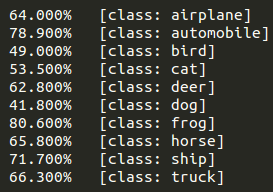
\includegraphics[width=1\textwidth]{\path/cifar-tanh.png} 
  \caption{Acc.= \textasciitilde 65\% f. di attivazione = TanH}
 \label{fig:training}
\end{subfigure}%
\begin{subfigure}{.5\textwidth}
  \centering
 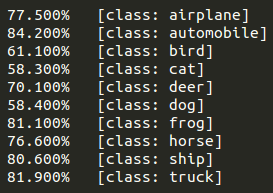
\includegraphics[width=1\textwidth]{\path/cifar-relu.png} 
  \caption{Acc.= \textasciitilde 73\% f. di attivazione = ReLU}
 \label{fig:validation}
\end{subfigure}
\caption{Percentuali di accuracy a seconda della funzione d'attivazione. La ReLU produce indubbiamente risultati migliori.}
\label{fig:relu}
\end{figure}
\\
%%%%% NEW PAGE FOR THE NEW FIGURES %%%% 
\newpage
\pagebreak
\medskip
\newpage

\begin{figure}[h!]
 \centering
 \includegraphics[width=1.0\textwidth]{\path/tensor-mode.jpg} 
 \caption{Fibers and slices of a tensor: fibers is an equivalent term for a tensor mode.}
 \label{fig:tensor-fibers}
\end{figure}

\begin{figure}[h!]
 \centering
 \includegraphics[width=1.0\textwidth]{\path/tucker-pass.jpg} 
 \caption{Tucker-2  decompositions  for  speeding-up  a generalized convolution. Each box corresponds to a 3-way tensor $X, Z, Z^' and Y$ in equation (\ref{eq:tucker1}-\ref{eq:tucker3}). Arrows represent linear mappings 
and illustrate each scalar value on the right is computed. Red tube, green cube and blue tube correspond to 
1x1, dxd and 1x1 convolution respectively.}
 \label{fig:tucker-pass}
\end{figure}


\begin{figure}[h!]
 \centering
 \includegraphics[width=1.0\textwidth]{\path/CPD.jpg} 
 \caption{Tensor decompositions for speeding up a generalized convolution. Each box correspond to a feature map stack within a CNN, (frontal sides are spatial dimensions). Arrows show linear mappings and demonstrate how scalar values on the right are computed. Initial full convolution (A) computes each element of the target tensor as a linear combination of the elements of a 3D subtensor that spans a spatial d × d window over all input maps. 
Jaderberg et al. (B) approximate the initial convolution as a composition of two linear mappings in which the intermediate mpa stack has R  maps, being R the rank of the decomposition. Each of the two-components 
computes each target value with a convolution based on a spatial window of size dx1 or 1xd in all input maps. Finally, CP-decomposition (C) by Lebedev et al. approximates the convolution as a composition of four smaller convolutions: the first and the last components compute a standard 1x1 convolution that spans all input maps while the middle ones compute a 1D grouped convolution \textbf{only on one} input map.}
 \label{fig:cpd-pass}
\end{figure}


